\documentclass[problem]{mcs}

\begin{pcomments}
    \pcomment{TP_a_bogus_tiling_induction}
    \pcomment{renamed from TP_A_Bogus_Induction}
    \pcomment{Written by EGM 01/30/13}
\end{pcomments}

\pkeywords{
induction
Tiles
Bill_Gates
bogus
logical_error
stategic_error
}

\begin{problem}
Frank Gehry has changed his mind.  Instead of the L-shaped tiles shown
in figure~\ref{fig:2Ltile}, he wants to use an odd offset pattern of
tiles (or its mirror-image reflection), as shown in
\ref{fig:offsettile}.  To prove this is possible, he uses reasoning
similar to the proof in~\ref{subsec:tile_induction}. However, unlike the
proof in the text, this proof is flawed.  Which part of the proof
below contains a logical error?

\begin{figure}

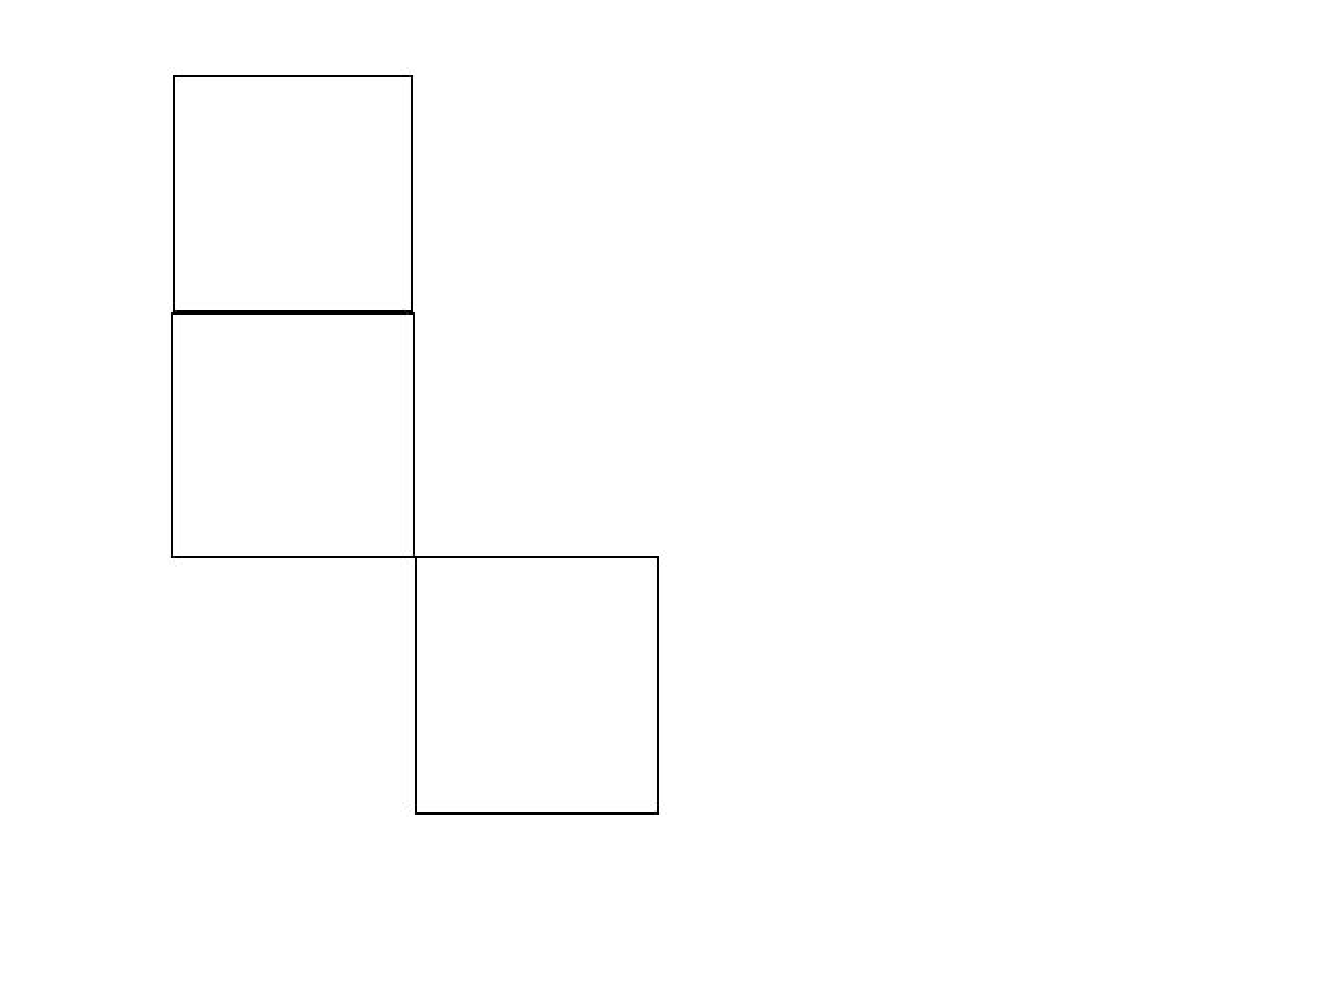
\includegraphics[height = 2in ]{Offset_tile}

\caption{Gehry's new tile.}
\label{fig:offsettile}
\end{figure}


\begin{falseclm*}\label{falsetiletheorem}
The proof is by induction.  Let $P(n)$ be the proposition that for
every location of Bill in a $2^n \times 2^n$ courtyard, there exists a
tiling of the remainder with the offset tile pattern.
\end{falseclm*}

\begin{falseproof}
\inductioncase{Base case}: $P(0)$ is true because Bill fills the
whole courtyard.

\inductioncase{Inductive step}: Assume that $P(n)$ is true for some
$n \geq 0$; that is, for every location of Bill in a $2^n \times 2^n$
courtyard, there exists a tiling of the remainder.  Divide the
$2^{n+1} \times 2^{n+1}$ courtyard into four quadrants, each $2^n
\times 2^n$.  One quadrant contains Bill (\textbf{B} in the diagram
below).  Place a temporary Bill (\textbf{X} in the diagram) in each of
the three squares lying near this quadrant as shown in
Figure~\ref{fig:bogustileimage}.

\begin{figure}

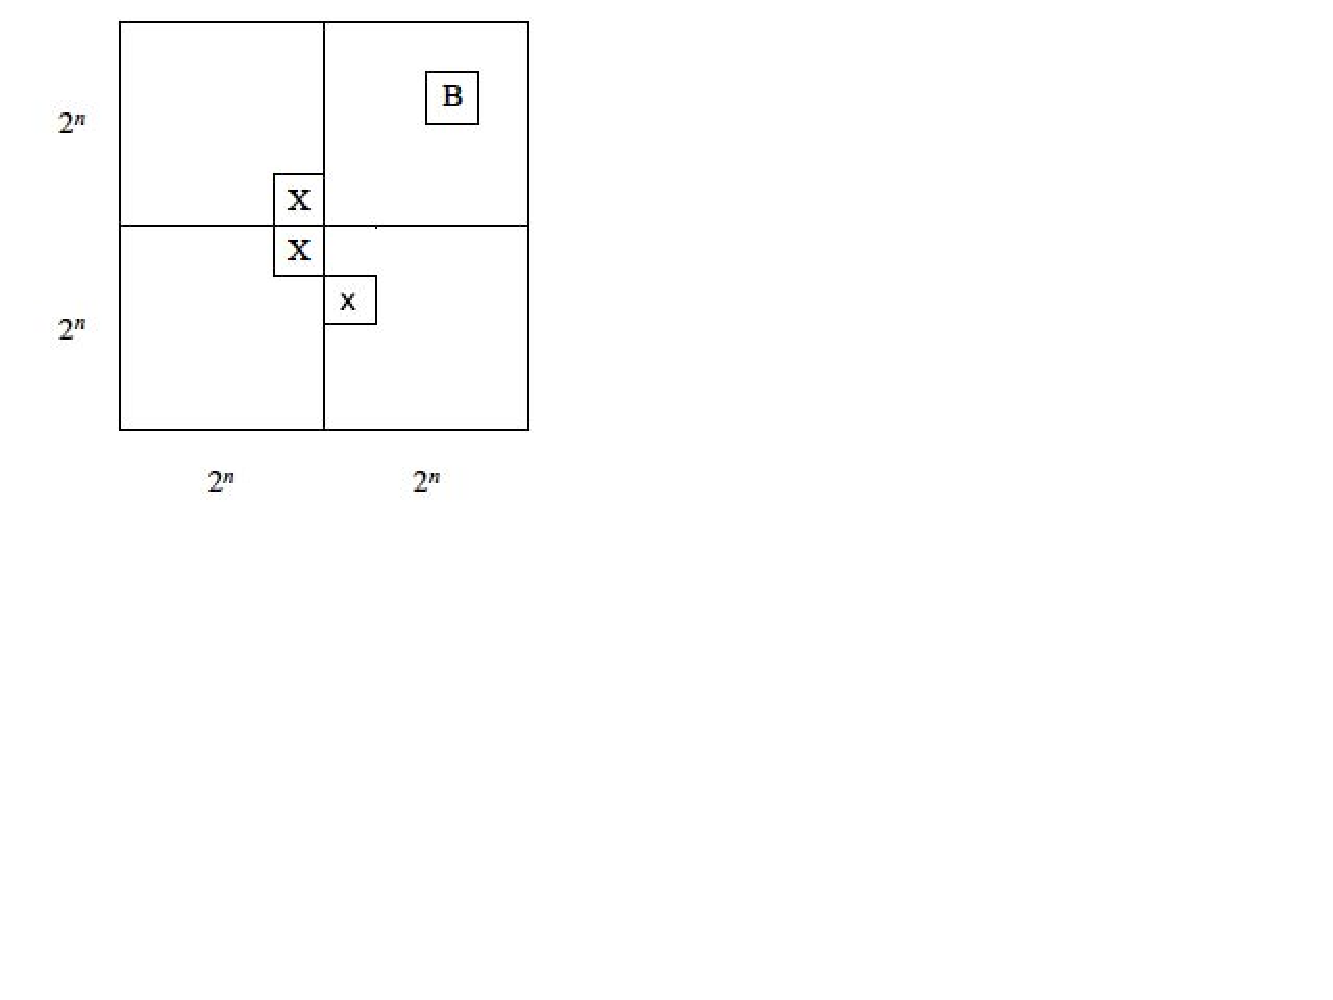
\includegraphics[trim = 0in 3in 5in 0in, clip, width = 3in]{Bogus_induction_step}

\caption{The induction hypothesis for the false theorem.}
\label{fig:bogustileimage}
\end{figure}

We can tile each of the four quadrants by the induction assumption.
Replacing the three temporary Bills with a single offset tile
completes the job.  This proves that $P(n)$ implies $P(n+1)$ for all
$n \geq 0$.  Thus $P(m)$ is true for all $m \in \nngint$, and the
ability to place Bill in the center of the courtyard follows as a
special case where we put Bill in a central square.
\end{falseproof}

%\hint Consider $n=1$.

\begin{solution}
The proof fails for $n=1$.  In this case, the diagram in
Figure~\ref{fig:bogustileimage} is misleading.  It makes it appear
that after the base case, that is, when $n>0$, there is room for an
offset tile near the middle of the plaza.  Now when $n>0$, there will
be room for an L-shaped tile, and when $n>1$ there will also be room
for the offset tile, but when $n=1$, there is no room for an offset
tile.  In fact, an offset tile is obviously too big to fit in a $2
\cross 2$ plaza, so the $2 \cross 2$ plaza can't be offset-tiled.
\end{solution}

\end{problem}

\endinput
